\chapter[Biology and Nonlinear Dynamics]{The Interplay of Biology and\\Dynamics of Nonlinear Systems}
\label{ch:biology-nonlinear}

\section{Introduction: Mechanics With a Biological State}

A golfer can arrive at nearly the same joint configuration and velocity with
different muscle activation, tendon strain and sensory estimates. Those states
need not produce the same subsequent motion. Geometry and rigid-body mechanics
remain essential, but positions and velocities alone may no longer close the
model. The additional state determines how a neural command becomes force, how
a disturbance propagates and which responses remain feasible before impact.

This is the useful connection between biology and nonlinear dynamics. Tissue
properties, neural feedback, task goals and contact conditions interact through
specific equations. Their interaction can support coordination; it can also
produce delay, instability, fatigue and estimation error. A biological label
does not decide which outcome occurs.

\begin{insight}[colframe=chapblue]{Three Questions That Must Be Kept Together}{bio-levels}
\begin{enumerate}
\item \textbf{Mechanics}: what forces and moments follow from the current
geometry, motion, tissue state and contact conditions?
\item \textbf{Control}: which excitation or actuator histories can change that
state within the remaining time and input limits?
\item \textbf{Evidence}: which measurements distinguish the proposed mechanism
from another model that produces the same observed movement?
\end{enumerate}
For a swing, the endpoint objective includes the clubhead's delivered position,
orientation and velocity, followed by collision dynamics. For a humanoid holding
a tool, it also includes grasp feasibility and balance. Neither objective is
specified by a single joint torque or a single measure of movement variability.
\end{insight}

\subsection{Bernstein, Constraints and the Scope of the Claim}

Having more muscle forces than independent joint moments makes force allocation
underdetermined unless additional information or assumptions are supplied. It
does not prove that the nervous system cannot coordinate the muscles, nor that
it must use a fixed small number of commands. A model's degrees of freedom,
actuators, measured EMG channels and task variables are different counts.

Newell grouped constraints into organism, task and environment~\cite{Newell1986}.
Bosch discusses stable and adaptable movement components in
sport~\cite{Bosch2020,Bosch2015}.
These frameworks motivate hypotheses; formal stability results require a
separate model and proof. Bosch's ``fluctuations''
can denote flexible task-dependent components; they are not, by definition,
expensive errors that must always be suppressed.

An intersection of feasible sets constrains possible states. It does not by
itself specify a vector field, an attractor or a controller. Two systems with
identical feasible configurations can have different inertia, dissipation and
feedback, and therefore different trajectories. Constraints-led practice and
predictive or feedback control are compatible descriptions at different levels.
Whether a golfer uses a particular internal representation requires evidence
beyond a successful dynamical model of the movement.

\section{Muscle, Tendon and Activation Dynamics}

\subsection{A Consistent Hill-Type Model}

Hill's shortening relation differs from later Hill-type muscle--tendon
models~\cite{Hill1938,millard2013flexing}. Declare which elements
are included, where their lengths are measured and how force is transmitted.
In an illustrative massless equilibrium model, a contractile element and passive
parallel element share the fiber length $l_f$. Their force is transmitted through
a series tendon, with pennation angle $\alpha$:
\begin{align}
F_f &= a F_0 f_L(l_f/l_0) f_V(\dot l_f/v_{\max})+F_{\mathrm{PE}}(l_f),
\label{eq:ch8:force-production}\\
F_t &= F_f\cos\alpha, \qquad
l_{\mathrm{MT}}(q)=l_t+l_f\cos\alpha.
\label{eq:ch8:hill-model}
\end{align}
Here $a\in[0,1]$ is activation, $F_0$ the reference active isometric fiber force,
$l_0$ the optimal fiber length, and $v_{\max}>0$ a shortening-speed scale.
The parallel force uses fiber length, not the total muscle--tendon length.
Pennation requires its own geometric law if it changes. Fiber and tendon forces
are not added as though series elements were parallel force sources.

A simple tension-only tendon law is
\begin{equation}
F_t=k_t[l_t-l_{\mathrm{slack}}]_+,
\qquad [z]_+=\max(z,0),
\label{eq:ch8:tendon-law}
\end{equation}
with $k_t$ in N/m. The extension is relative to tendon slack length, not muscle
length. This piecewise linear law is a teaching approximation; physiological
tendon models can include a nonlinear toe region and hysteresis. Series
equilibrium and path length together determine fiber velocity or require an
implicit solve. Slack tendon and near-zero activation need careful numerical
treatment rather than division by a vanishing active-force term.

\begin{figure}[htbp]
\centering
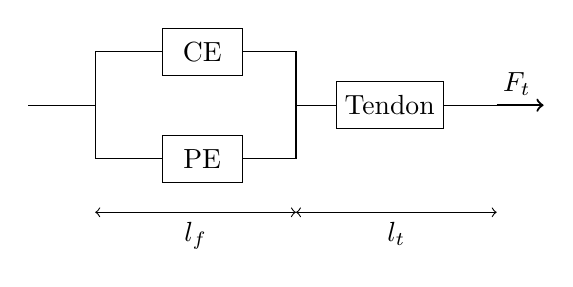
\begin{tikzpicture}[x=0.85cm,y=0.85cm]
\draw (0,0)--(1,0)--(1,0.8)--(2,0.8);
\draw (2,0.45) rectangle (3.2,1.15);
\node at (2.6,0.8) {CE};
\draw (3.2,0.8)--(4,0.8)--(4,0);
\draw (1,0)--(1,-0.8)--(2,-0.8);
\draw (2,-1.15) rectangle (3.2,-0.45);
\node at (2.6,-0.8) {PE};
\draw (3.2,-0.8)--(4,-0.8)--(4,0)--(4.6,0);
\draw (4.6,-0.35) rectangle (6.2,0.35);
\node at (5.4,0) {Tendon};
\draw (6.2,0)--(7,0);
\draw[<->] (1,-1.6)--(4,-1.6);
\node[below] at (2.5,-1.6) {$l_f$};
\draw[<->] (4,-1.6)--(7,-1.6);
\node[below] at (5.5,-1.6) {$l_t$};
\draw[->,thick] (7,0)--(7.7,0);
\node[above] at (7.3,0) {$F_t$};
\end{tikzpicture}
\caption{Parallel Fiber Elements and a Series Tendon. The Schematic Uses Zero
Pennation; a Pennate Model Must Project Fiber Force and Length Consistently.}
\label{fig:ch8:hill-model}
\end{figure}

\subsection{Length and Velocity Conventions That Can Be Checked}

Let $\nu=\dot l_f/v_{\max}$, so shortening means $\nu<0$.
One explicit illustrative pair of normalized curves is
\begin{align}
f_L(\ell)&=\exp\left[-\left(\frac{\ell-1}{w}\right)^2\right],\quad w>0,
\label{eq:ch8:force-length}\\
f_V(\nu)&=
\begin{cases}
\dfrac{1+\nu}{1-\nu/c},&-1\leq\nu\leq0,\\[4pt]
1+(N-1)\dfrac{\nu}{d+\nu},&\nu>0,
\end{cases}
\quad c,d>0,\quad N>1.
\label{eq:ch8:force-velocity}
\end{align}
These equations define the example, not a universal parameter fit or Hill's
original eccentric law. They give $f_V(-1)=0$, $f_V(0)=1$, and an eccentric
limit $N$. The shortening branch increases with $\nu$; faster shortening
therefore reduces force. Its derivative at zero is $1+1/c$. Choosing
$d=(N-1)/(1+1/c)$ also matches the eccentric branch's derivative there.
Outside the stated domain, choose and validate an extension rather than letting
negative active tension silently enter a simulation.

For $c=0.25$, $N=1.5$ and $d=0.1$, $f_V(-0.5)=1/6$ and
$f_V(0.1)=1.25$. At $a=0.5$, $F_0=1000$ N and optimal length, active fiber
force is respectively $83.33$ N and $625$ N. These are chosen model numbers,
not measured human values. Passive force and pennation still affect tendon
force. Total force at a long fiber length can exceed active isometric force
because the passive element contributes; the active force--length peak alone
does not bound the total tension.

\subsection{Zero Excitation Retains the Activation History}

Excitation $u$ and activation $a$ are different variables. For a constant
activation time scale $\tau_a>0$, a simple example is
\begin{equation}
\dot a=(u-a)/\tau_a,\qquad 0\leq u\leq1.
\label{eq:ch8:activation}
\end{equation}
If $u$ is set to zero at $t_0$, then
$a(t)=a(t_0)\exp[-(t-t_0)/\tau_a]$. Active force generally persists while
activation decays. Real activation/deactivation dynamics can require different
time scales and nonlinearities. With activation, fiber length and other internal
states $z$, a closed model uses $x=(q,v,a,z)$, not only $x=(q,v)$.

For muscle path lengths $l_{\mathrm{MT}}(q)$, define
$J_l=\partial l_{\mathrm{MT}}/\partial q$. Positive tendon tension pulls toward
shorter path length, giving generalized muscle load $-J_l^T F_t$:
\begin{align}
M(q)\dot v+h(q,v)&=-J_l(q)^TF_t(x)+Q_{\mathrm{ext}}+A(q)^T\lambda,
\label{eq:ch8:body-dynamics}\\
\dot q&=v,\qquad \dot z=\psi(x),\qquad
Av=0.
\end{align}
Here generalized coordinates are chosen so $\dot q=v$; other representations
need their kinematic map. $h$ includes the declared gravity and velocity terms,
and $\lambda$ enforces the current independent ideal constraints. Ground friction,
grasp limits and changing contact modes need additional conditions.

With constant $\tau_a$ and no other direct excitation dependence, the augmented
system is control-affine: $\dot x=f(x)+G(x)u$. Excitation enters the activation
rows; its influence on acceleration develops through the state. The drift
$f$ at $u=0$ includes existing activation, tendon strain and constraint response.
Holding a nonzero baseline command instead defines another vector field. It is
legitimate to study that field, but it must not be called fully passive or free
of ongoing energetic cost.

\subsection{Preflex Response and Tendon Energy}

An intrinsic mechanical response can precede a newly evoked neural response.
At a fixed activation and around a specified state, a local approximation is
\begin{equation}
\delta F_f\simeq K_f\delta l_f+D_f\delta\dot l_f.
\label{eq:ch8:preflex-force}
\end{equation}
The coefficients depend on operating point and history, not just activation.
This approximation is often associated with the preflex concept~\cite{Loeb1995}.
It introduces no new neural-loop delay; that does not imply instantaneous global
force transmission, an inactive nervous system, or guaranteed stability.
The sign and size of incremental stiffness, tendon compliance, limb geometry
and contact determine the resulting motion.

For example, a damped inverted pendulum near upright obeys
\begin{equation}
I\ddot\theta+D\dot\theta+(K-mgh)\theta=0.
\label{eq:ch8:posture-stability}
\end{equation}
With $I>0$ and $D>0$, this linear model is asymptotically stable only when
$K>mgh$. Positive tissue stiffness is insufficient if it is smaller than the
destabilizing gravitational term. Direct human standing measurements by Loram
and Lakie found intrinsic ankle stiffness insufficient for stability in their
protocol~\cite{LoramLakie2002}. This is a useful counterexample to a general
claim that baseline muscle tone automatically stabilizes posture. Spinal
circuits are part of the CNS; anesthesia does not imply elimination of every
reflex. Neither claim is needed to explain a mechanical preflex.

For the elastic law above,
\begin{equation}
E_t=\tfrac12 k_t[l_t-l_{\mathrm{slack}}]_+^2,
\qquad \dot E_t=F_t\dot l_t
\label{eq:ch8:tendon-energy}
\end{equation}
away from the switching point. A chosen $k_t=20{,}000$ N/m and 0.02 m
extension store 4 J at 400 N. Releasing 4 J in 0.02 s supplies 200 W of average
recoil power in this ideal example. The energy had to be loaded earlier;
recoil changes the timing of power without creating energy. Fiber work,
skeletal work, tendon storage and losses must close one balance. There is no
universal 50\% tendon contribution to jumping or striking, and an elastic
element is not generally equivalent to rescaling time in a rigid-body solution.

For a golf swing, a catapult hypothesis therefore needs a measured or bounded
strain history and release timing. A compliant robot actuator needs the same
accounting. More compliance can improve a specified objective or impair force
bandwidth, precision and contact control; the answer depends on the task.

\section{Attractors and Coordination Transitions}

\subsection{What Stability Does and Does Not Establish}

For a declared autonomous closed-loop system, we use an asymptotically stable
attractor to mean a compact invariant set that is Lyapunov stable and attracts
some neighborhood. Lyapunov stability means sufficiently small disturbances
remain small; attraction additionally concerns convergence to the set.
Definitions of more general attractors differ, so minimality and a single
negative exponent should not be substituted for these conditions.

Attraction to a periodic orbit is distinct from convergence to one time-stamped
trajectory on that orbit. A stable autonomous limit cycle has a neutral phase
direction, with a zero Lyapunov exponent and a unit Floquet multiplier; its
transverse multipliers can lie inside the unit circle. Nearby motions can retain
a phase offset while approaching the same orbit. A chaotic attractor can attract
trajectories to its set while separating nearby trajectories within that set.
Finite-time growth, asymptotic exponents and basin size answer different questions.

These distinctions matter in golf. A repeatable swing is a finite-duration
movement ending in contact, not automatically a limit cycle or equilibrium.
An appropriate analysis can use a trajectory tube, terminal error, input limits
and impact-event sensitivity. A phase error that is harmless for convergence to
a periodic gait can be consequential when club and ball must meet at one time.

An attractor can be generated by passive mechanics, constant powered actuation,
neural feedback or a robot controller. Its existence does not identify which
mechanism supplies stability, how much power is consumed or whether a new task
can be accommodated. A passive downhill walker draws energy from gravity;
an actively stabilized posture can consume energy without moving. A finite
feedforward maneuver need not be an attractor to meet an error tolerance.

\begin{example}[colframe=chapblue]{A Stable Orbit With a Neutral Phase}{bio-limit-cycle}
On an annulus around $r=1$, consider $\dot r=1-r$, $\dot\theta=\omega>0$.
Radial deviations decay as $e^{-t}$, but two solutions' angular difference
remains constant. The orbit $r=1$ attracts nearby states although their
time-matched Euclidean separation need not tend to zero. Transverse recovery
and phase recovery must therefore be measured separately.
\end{example}

\subsection{A Cost Crossing Is Not a Dynamical Bifurcation}

A dynamical bifurcation changes the qualitative behavior of a vector field or
return map as a parameter varies. Two metabolic cost curves crossing does not
show that either gait loses dynamical stability. Even in the simple chosen
costs $C_1(v)=1+v^2$ and $C_2(v)=2+v^2/2$, the crossing at $v=\sqrt2$
says only which algebraic cost is smaller. It supplies no equations for a gait.
An observed walk--run transition can be investigated using energetic, mechanical,
perceptual and stability hypotheses; matching one transition speed does not
distinguish them. These teaching curves are dimensionless examples, not fitted
human metabolic laws.

Likewise, a coordination variable and an experimentally adjusted ``control
parameter'' are not necessarily a plant state and actuator input in the
control-theory sense. The relationship must be derived or fitted. Frequency
may alter several physiological and mechanical processes at once.

\subsection{The Haken--Kelso--Bunz Model With Its Correct Transition}
\label{sec:bio-hkb}

In the classic bimanual experiment, increasing cycling frequency can cause the
initial anti-phase mode to switch to in-phase coordination, using the authors'
homologous-muscle phase convention~\cite{HakenKelsoBunz1985}. Symmetric movements
toward and away from the body's midline can be in-phase even though the hands'
world-coordinate velocities point in opposite directions. Define the measured
phase before using ``same direction'' as a substitute.

The standard reduced deterministic phase equation is first order:
\begin{align}
\dot\phi&=-a_H\sin\phi-2b_H\sin(2\phi)=-V'(\phi),
\label{eq:ch8:hkb-model}\\
V(\phi)&=-a_H\cos\phi-b_H\cos(2\phi),\qquad a_H,b_H>0.
\end{align}
The potential is a reduced dynamical construction, not metabolic or mechanical
energy. For fixed parameters, $\dot V=-[V'(\phi)]^2\leq0$. Linearizing at the
two coordination modes gives
\begin{equation}
\lambda_0=-a_H-4b_H<0,\qquad
\lambda_\pi=a_H-4b_H.
\label{eq:ch8:hkb-stability}
\end{equation}
Thus in-phase $\phi=0$ remains locally stable, whereas anti-phase $\phi=\pi$
is stable only for $b_H/a_H>1/4$. If the ratio decreases through $1/4$ as
cycling frequency increases, anti-phase loses stability. A chosen frequency
law is required before assigning a transition frequency in Hz. A forced
second-order phase oscillator is a different model requiring its own derivation.

For $a_H=1$ s$^{-1}$, changing $b_H$ from 0.5 to 0.2 s$^{-1}$ changes
$\lambda_\pi$ from $-1$ to $+0.2$ s$^{-1}$ while $\lambda_0$ remains negative.
Exactly $\phi=\pi$ is an equilibrium even after losing stability: a numerical
experiment must include a small perturbation or a declared noise process to
observe departure. Near the transition, slow recovery and noise-induced switching
can complicate identification of the deterministic threshold.

\begin{figure}[htbp]
\centering
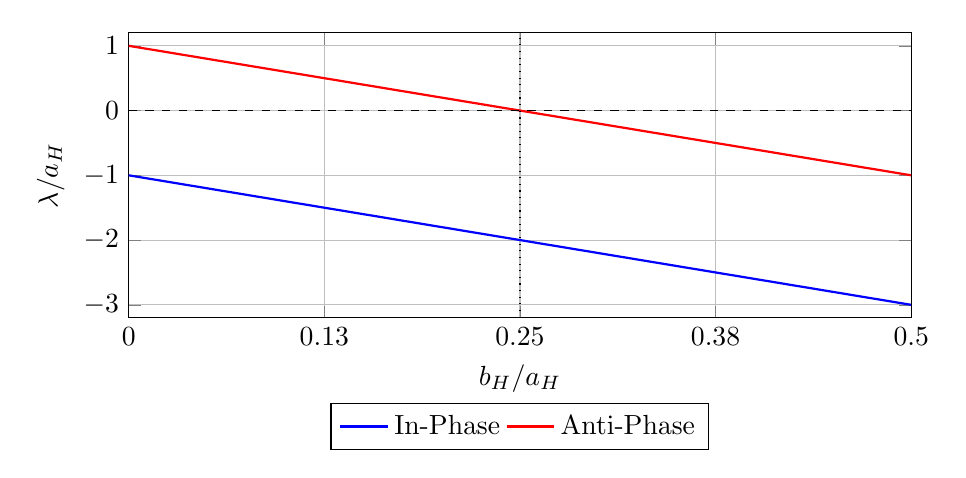
\begin{tikzpicture}
\begin{axis}[width=0.95\linewidth,height=5.2cm,
xmin=0,xmax=0.5,ymin=-3.2,ymax=1.2,
xlabel={$b_H/a_H$},ylabel={$\lambda/a_H$},
xtick={0,0.125,0.25,0.375,0.5},ytick={-3,-2,-1,0,1},
legend style={at={(0.5,-0.3)},anchor=north,legend columns=2},
grid=major]
\addplot[blue,thick,domain=0:0.5] {-1-4*x};
\addlegendentry{In-Phase}
\addplot[red,thick,domain=0:0.5] {1-4*x};
\addlegendentry{Anti-Phase}
\addplot[black,dashed,forget plot] coordinates {(0,0) (0.5,0)};
\addplot[black,dotted,forget plot] coordinates {(0.25,-3.2) (0.25,1.2)};
\end{axis}
\end{tikzpicture}
\caption{Local Phase Stability in the HKB Reduction. Negative Rates Indicate
Recovery; Anti-Phase Loses Stability as the Ratio Falls Below One Quarter.}
\label{fig:ch8:hkb-bifurcation}
\end{figure}

The reduced model explains an experimental coordination transition without an
explicit discrete mode-selection command in its equations. It does not show
that neurons are absent, that the brain never predicts trajectories or that
golf timing follows the same phase law. In a swing, a proposed collective
variable needs a measurement definition, fitted dynamics and tests under
perturbations and altered tempo. A recognizable pattern is a starting point
for that work, not its causal conclusion.

\section{Synergies, Task Geometry and Control Authority}

\subsection{What a Low-Dimensional Fit Establishes}

A spatial muscle-synergy model approximates an EMG or activation matrix
$U\in\mathbb R^{p\times N}$ by $WC$, with $W\in\mathbb R^{p\times k}$ and
$C\in\mathbb R^{k\times N}$. Nonnegative factorization usually imposes
$W,C\geq0$. Specify preprocessing, normalization, muscles, tasks and rank
selection; EMG is not a direct measurement of muscle force.
\begin{equation}
\mathrm{VAF}_{\mathrm{uncentered}}
=100\left(1-\frac{\|U-WC\|_F^2}{\|U\|_F^2}\right)\%,
\qquad \|U\|_F>0.
\label{eq:ch8:vaf}
\end{equation}
The percentage multiplies the entire bracket. A centered variance definition
uses a different denominator and must be named. High reconstruction quality
is a property of the dataset and fit, not proof of a neural module or a
universal number of synergies.

Kutch and Valero-Cuevas supplied counterexamples in which biomechanics
produces low-dimensional activation patterns without fixed neural grouping
\cite{KutchValeroCuevas2012}. Such alternatives do not establish that neural
synergies never exist. They show why a causal claim needs task variation,
perturbation, held-out prediction and comparison with independently controlled
muscles. A useful robot policy may intentionally restrict its inputs to
synergies even when the corresponding human mechanism remains unresolved.

\subsection{A Task Level Set and Its Tangent Space}

For a smooth task map $y=h(q)$ and target $y_*$, the exact task-preserving set is
\begin{equation}
\mathcal M_{y_*}=\{q:h(q)=y_*\}.
\label{eq:ch8:ucm}
\end{equation}
At a regular point $\bar q$ with rank-$r$ Jacobian $J=Dh(\bar q)$, its tangent
space is $\ker J$ and has dimension $n-r$. The local uncontrolled-manifold
analysis uses this linear approximation~\cite{ScholzSchoner1999}. A finite step
in a tangent direction generally leaves the curved level set:
\begin{equation}
h(\bar q+\delta q)-h(\bar q)
=J\delta q+\tfrac12 D^2h(\bar q)[\delta q,\delta q]
+O(\|\delta q\|^3).
\end{equation}
For $h(q)=q_1^2+q_2^2$, $\bar q=(1,0)$ and $\delta q=(0,0.1)$,
$J\delta q=0$ but the task value increases from 1 to 1.01. A singular point
requires a separate analysis; a changing Jacobian rank invalidates one fixed
dimension formula across the whole region.

Using a declared Euclidean metric, let $P_N=I-J^\dagger J$ and
$P_R=J^\dagger J$. For joint-deviation covariance $\Sigma$, dimension-normalized
variances are
\begin{equation}
V_{\mathrm{UCM}}=\frac{\operatorname{tr}(P_N\Sigma)}{n-r},\qquad
V_{\mathrm{ORT}}=\frac{\operatorname{tr}(P_R\Sigma)}{r},
\quad 0<r<n.
\label{eq:ch8:ucm-variance}
\end{equation}
Coordinates mixing lengths and angles require meaningful scaling or another
metric. For isotropic noise $\Sigma=\sigma^2I$, both normalized variances equal
$\sigma^2$; redundancy alone does not give a ratio greater than one. Repeated
trials also need alignment, a task definition and a treatment of measurement
noise. More variance in the tangent directions supports a particular
task-stabilization hypothesis; it does not establish that these directions
are neurologically uncontrolled or irrelevant to every goal.

In golf, a null direction for hand position may change face orientation, shaft
strain, grip loading or a later collision. The chosen output should therefore
reflect the actual question. Kinematic task-preserving variations and muscle
activation synergies live in different spaces; relating them requires muscle
geometry and dynamics rather than identifying the two subspaces by name.

\subsection{Instantaneous Rank Is Not Controllability}

If an input policy imposes $u=Wc$ in $\dot x=f(x)+G(x)u$, the instantaneous
input map is $GW$, with rank at most $k$. Nonnegative and bounded amplitudes
further limit the feasible directions to a cone or bounded set. This does not
mean that the other state directions are uncontrollable over time.

For the double integrator $\dot q=v$, $\dot v=u$, the instantaneous input
matrix is $B=(0,1)^T$, but
\begin{equation}
A=\begin{pmatrix}0&1\\0&0\end{pmatrix},\qquad
[B,AB]=\begin{pmatrix}0&1\\1&0\end{pmatrix}
\label{eq:ch8:controllability-example}
\end{equation}
has rank two. Drift transports the input's effect into position. Along a
general nominal motion, use the linearized pair $A(t),B(t)$ and, where
appropriate, its finite-horizon Gramian. Nonlinear accessibility, finite-time
reachability and controllability under bounds are distinct additional questions.

Nor does a direction invisible in the current output remain unobservable.
For the same double integrator with output $y=q$, velocity is initially in
$\ker C$, $C=(1,0)$, yet $[C^T,(CA)^T]^T$ has rank two. Position measured over
time reveals velocity in the ideal model. There is no theorem that discarded
synergy directions must coincide with an unobservable UCM. The practical test
is whether the restricted policy can meet the chosen task and disturbance
tolerances within its available time and force limits.

\section{Impedance and Co-Contraction}

\subsection{Force, Displacement and Velocity Ports}

For a local scalar perturbation model around a fixed operating point,
\begin{equation}
M\delta\ddot x+D\delta\dot x+K\delta x=\delta F,
\qquad M,D,K>0,
\label{eq:ch8:impedance-time}
\end{equation}
the zero-initial-condition Laplace relations are
\begin{align}
S(s)&=\frac{\delta F(s)}{\delta X(s)}=Ms^2+Ds+K,
\label{eq:ch8:dynamic-stiffness}\\
Z(s)&=\frac{\delta F(s)}{\delta V(s)}=Ms+D+K/s,
\label{eq:ch8:impedance-laplace}\\
H(s)&=\frac{\delta X(s)}{\delta F(s)}=\frac1{Ms^2+Ds+K}.
\end{align}
$S$ is dynamic stiffness (N/m); $Z$ is mechanical impedance (N\,s/m); $H$
is displacement compliance. Some robotics literature uses ``impedance control''
for enforcing the complete mass--damping--stiffness relation. Naming that strategy
does not remove the distinction between the transfer functions and their units.
Multi-axis impedance needs matrices, a frame and a power-consistent port.

The natural frequency is $\omega_n=\sqrt{K/M}$ and damping ratio
$\zeta=D/(2\sqrt{MK})$. Increasing $K$ at fixed $D$ raises $\omega_n$ but lowers
$\zeta$. For the chosen $M=1$ kg, $D=10$ N\,s/m and $K=100$ N/m,
$\omega_n=10$ rad/s and $\zeta=0.5$. Increasing $K$ to 400 N/m doubles the
natural frequency and halves the damping ratio. A faster natural time scale
does not guarantee less overshoot, smaller contact forces or better performance.

\subsection{How Muscle Forces Contribute to Joint Stiffness}

At fixed activation and internal-state assumptions, take
$\tau(q)=-\sum_i F_i(l_i(q))\nabla l_i(q)$. Linearized restoring stiffness is
\begin{equation}
K_q=-\frac{\partial\tau}{\partial q}
=\sum_i\left[
k_i\nabla l_i\nabla l_i^T+F_i\nabla^2l_i\right],
\qquad k_i=\frac{\partial F_i}{\partial l_i}.
\label{eq:ch8:cocontraction-stiffness}
\end{equation}
The first term is material stiffness transmitted through moment arms; the
second is geometric stiffness from loaded, changing geometry. Muscle--tendon
series compliance changes the effective $k_i$. Coupled muscle dynamics,
reflexes and active feedback require a frequency-dependent extension.

In a chosen one-joint model with constant opposing moment arms of 0.03 m,
equal forces of 100 N produce zero net torque. If both effective longitudinal
stiffnesses are 10,000 N/m, the joint stiffness is
$2(0.03)^2(10{,}000)=18$ N\,m/rad. The antagonists carry real load even though
their net torque cancels. Equal activation need not produce equal opposing
torques when muscle sizes, lengths or moment arms differ.

Hogan's analysis and forearm-posture experiment support a role for antagonist
coactivation in impedance modulation~\cite{Hogan1984}. They do not establish
a universal stiffness proportional to target uncertainty. Target uncertainty,
external force disturbances, observation noise and activation-dependent noise
enter different parts of a control problem. Increasing stiffness can resist
a force disturbance while increasing the force caused by a position error
against a stiff environment. The disturbance and the scored outcome must be named.

\subsection{An Explicit Optimization Example}

For a quasistatic scalar model $e=w/K$ with zero-mean force disturbance of
variance $\sigma_F^2$, suppose a designer chooses the surrogate
\begin{equation}
J(K)=\frac{\sigma_F^2}{K^2}+\rho K^2,\qquad
0<K_{\min}\leq K\leq K_{\max},\quad\rho>0.
\label{eq:ch8:impedance-cost}
\end{equation}
Weights carry the units needed to compare the terms. The first term is expected
squared displacement; the second is an assumed stiffness penalty, not measured
metabolic energy. Before applying bounds, differentiation gives
\begin{equation}
K_0=(\sigma_F^2/\rho)^{1/4},\qquad
K^*=\operatorname{clip}(K_0,K_{\min},K_{\max}).
\label{eq:ch8:optimal-k}
\end{equation}
For $\sigma_F=10$ N, $\rho=10^{-6}$ m$^4$/N$^2$ and bounds
20--150 N/m, $K^*=100$ N/m. Four times the force standard deviation would
make the unconstrained optimum 200 N/m and the bounded optimum 150 N/m.
Maximum feasible stiffness can therefore be optimal for a stated task. Changing
the penalty, disturbance spectrum or dynamics changes the result; there is
no general linear ``signal-to-noise'' stiffness law.

For the stable compliance $H$ above,
$\|H\|_\infty=\sup_\omega|H(i\omega)|$ measures a frequency-domain gain and
the induced $L_2$ gain under the usual zero-initial-condition assumptions.
It does not guarantee bounded output for arbitrary unlimited disturbances or
robustness to unspecified model uncertainty. For this scalar system,
\begin{equation}
\|H\|_\infty=
\begin{cases}
1/K,&\zeta\geq1/\sqrt2,\\[2pt]
1/[2\zeta K\sqrt{1-\zeta^2}],&0<\zeta<1/\sqrt2.
\end{cases}
\label{eq:ch8:hinfinity}
\end{equation}
The dynamic-stiffness polynomial $S$ instead grows without bound at high
frequency; it is not the stable proper disturbance-to-displacement transfer
whose finite norm was intended. In a real controller, sensing, filters, delay,
contact and actuator dynamics determine the relevant closed-loop transfer.

\subsection{Mechanical Work and Metabolic Cost}

The local passive model stores
$E=\tfrac12M\delta\dot x^2+\tfrac12K\delta x^2$ and, for constant $M,K$,
obeys $\dot E=\delta F\delta\dot x-D\delta\dot x^2$.
If stiffness is varied, an additional $\tfrac12\dot K\delta x^2$ term enters
the energy balance. An actively changed spring parameter can supply energy;
passivity cannot be inferred from positive instantaneous $K$ alone.

Physiological metabolic cost also depends on activation, contraction history,
force and velocity, tissue properties and the selected metabolic model.
It is not generally proportional to $\int K\,dt$, net joint work, or squared
inverse-dynamics torque. A golfer can have low net wrist torque while opposing
muscles are loaded. A robot can hold a load with zero joint work while its
motor dissipates electrical energy. Report the measured or modeled cost actually
used; mechanical cancellation does not make physiological effort disappear.

\section{Pre-Stress and Stability of Interacting Subsystems}

\subsection{What a Tensegrity Analogy Can Contribute}

Pre-stress means an internal load state present before an additional perturbation.
A self-stress in a free structural model balances internally without external
nodal load. More generally, a loaded structure is linearized around an equilibrium
that includes its external loads. Neither definition says that ``internal forces
exceed external forces''; these are different force collections, not one scalar
comparison.

For a declared elastic potential $U(q)$, the constrained tangent stiffness comes
from the appropriate second variation of total potential at equilibrium. Material
and geometric contributions both matter, as in the preceding muscle-path formula.
Preloading can stiffen some directions and soften others, including buckling.
Equilibrium force balance alone does not prove stability.

Tensegrity models can help formulate questions about distributed load paths.
Anatomical bones also experience bending, shear and joint-contact forces, while
muscles, tendons and fascia have distributed geometry and constitutive behavior.
A cell-scale or ideal strut--cable model is not by itself validation of a
whole-body architecture. Rigid-body multibody models can already include muscle
forces, compliance and loaded constraints; these modeling approaches need not
be treated as mutually exclusive.

For golf, useful questions concern the force path from ground through legs,
trunk, arms and grip, and the resulting tangent response under a defined
perturbation. Muscle tone supplies force and may change that response; it is
not separate from force generation. A proposed fascia-mediated mechanism must
predict an observable effect beyond what the competing joint/contact model
already explains. A humanoid comparison likewise needs a specified structure,
actuation and contact model, rather than an anatomical analogy alone.

\subsection{Why Stable Parts Can Form an Unstable Whole}

Organizing analysis into tissue, intermuscular and task levels is useful.
Their time scales overlap, however, and their couplings must remain in the
equations. A spinal feedback loop is a CNS process, and faster mechanics does
not eliminate sensing, prediction or adaptation. Separate stability does not
guarantee that the sum of the levels' Lyapunov functions is a composite
certificate: coupling terms must also be controlled.

\begin{example}[colframe=chapblue]{An Unstable Interconnection of Stable Scalar Parts}{bio-coupling}
Consider
\begin{equation}
\dot z_1=-z_1+2z_2,\qquad \dot z_2=-z_2+2z_1.
\label{eq:ch8:unstable-coupling}
\end{equation}
Each isolated equation decays when the other state is fixed at zero. The
coupled matrix has eigenvalues $1$ and $-3$. For
$V=(z_1^2+z_2^2)/2$, $\dot V=-z_1^2-z_2^2+4z_1z_2$ is positive at
$z_1=z_2\ne0$. Separate stability has not controlled the feedback interaction.
\end{example}

\begin{theorem}[A Sufficient Composite Decay Condition]
\label{thm:nested-lyapunov}
Suppose positive-definite local functions $V_i$ for a common equilibrium satisfy,
on a specified neighborhood,
\[
\dot V_i\leq-\alpha_i\|z_i\|^2+
\sum_{j\ne i}\gamma_{ij}\|z_i\|\|z_j\|,
\qquad \alpha_i>0,\quad\gamma_{ij}\geq0.
\]
If weights $w_i>0$ make the symmetric matrix with entries
\[
S_{ii}=w_i\alpha_i,\qquad
S_{ij}=-\tfrac12(w_i\gamma_{ij}+w_j\gamma_{ji})
\]
positive definite, then $V=\sum_i w_iV_i$ has strictly negative derivative
away from the equilibrium in that neighborhood. With the usual regularity
and local positive-definiteness bounds, it proves local asymptotic stability.
\end{theorem}
\begin{proof}
Set $r_i=\|z_i\|$. Summing the derivative bounds gives
$\dot V\leq-r^TSr\leq-\lambda_{\min}(S)\|r\|^2$.
Small enough sublevel sets remain inside the neighborhood; the Lyapunov
criterion then applies. A global conclusion would require global hypotheses.
\end{proof}

For three scalar levels with diagonal decay one and symmetric neighbor coupling
0.2, the decay matrix has smallest eigenvalue $1-0.2\sqrt2\simeq0.7172>0$.
This chosen example passes the condition. It is not an estimate of a nervous
system's coupling strength. Other systems may need input-to-state stability,
small-gain, passivity or singular-perturbation analysis. For contact switches,
also check reset-induced changes in the certificate; continuous decay between
events is not a complete hybrid stability proof.

The resulting research claim is specific: suitable coupling and feedback can
make distributed stabilization work. A hierarchy is an analysis strategy,
not automatic protection from dimensionality, delay or instability.

\section{Building and Testing a Coupled Movement Model}

\subsection{Choose the Model for the Question}

Inverse dynamics recovers the net generalized loads consistent with specified
kinematics, inertia and external loads. It does not inherently assume that
muscle activation is instantaneous or that tendons are rigid: those assumptions
belong to a chosen actuator model. Recovering a joint moment does not identify
the individual muscle forces producing it. Ballistic movements can be particularly
sensitive to activation history, elasticity and contact timing; speed alone
does not justify ignoring those states.

A practical model comparison starts with a rigid-body net-load model, then
adds only the states needed to answer the question. A muscle-driven model can
add activation, fiber and tendon dynamics; a humanoid actuator model can add
motor current, transmission compliance and control delay. Flexible shafts and
grips require corresponding deformation states. Both versions should retain
the same task, initial-condition specification and external-load convention.

Check equilibrium, power balance, force bounds, constraint residuals and numerical
convergence before interpreting differences. A more elaborate model can fit
more observations while being less identifiable. Adding springs or feedback
does not guarantee useful attractors, favorable energy transfer or better
predictions. Compare the simplest competing models against held-out data.

\subsection{Identification Requires More Than a Motion Fit}

Let measurements satisfy $y_k=\mathcal H(x(t_k),\theta)+\epsilon_k$, with
parameters $\theta$. The local sensitivity matrix
\begin{equation}
\mathcal S_{kj}=\frac{\partial y_k}{\partial\theta_j}
\label{eq:ch8:identification}
\end{equation}
reveals combinations distinguishable in the selected experiment. When columns
are nearly dependent, different parameters can compensate for one another.
Measurement covariance, parameter scaling and model discrepancy all affect
the interpretation. A successful optimizer does not establish physiological
uniqueness or remove uncertainty.

Joint motion and ground reactions constrain net mechanics. EMG adds timing and
activation-related evidence with its own calibration limitations. Ultrasound
or other tissue measurements can constrain fiber or tendon behavior when the
measurement is appropriate. Perturbation experiments can separate stiffness,
damping and delayed feedback more effectively than repeated unperturbed motion.
No fixed parameter count guarantees identifiability, and imaging is not uniformly
invasive. Specify what each measurement adds and what remains inferred.

For learning and fatigue, parameters or policies may change across trials.
Separate within-trial state estimation from across-trial adaptation. A model
that refits each swing independently can conceal a failure to predict how a
changed grip, tempo, load or support condition changes the response.

\subsection{A Golf and Humanoid Experiment Ladder}

\begin{enumerate}
\item \textbf{Define the delivered state}. Record the clubhead or tool frame,
reference point, contact event and task tolerance. State whether the objective
is face control, speed, balance, disturbance recovery or a combination. Joint
angles alone do not specify all of these outcomes.
\item \textbf{Define comparable initial conditions}. Match or estimate posture,
velocity, activation and elastic state. Distinguish a new command from a
changed starting state. A zero-excitation continuation preserves the existing
activation and strain history; it is not an instruction to make the person
instantaneously relaxed.
\item \textbf{Apply a declared disturbance}. Vary tool inertia, support,
grip loading or a measured external perturbation within an appropriate protocol.
Specify the time and direction. Disturbances applied before and near impact
probe different available correction horizons.
\item \textbf{Measure both task and internal response}. Compare delivered
state, phase error, hand/ground loads and relevant activation or strain evidence.
A successful endpoint with larger opposing forces may trade robustness for
effort. Lower joint torque alone cannot decide whether that trade occurred.
\item \textbf{Compare mechanisms}. Test a net-load model, an augmented tissue
or actuator model, and alternative feedback policies using the same scored
data. Report prediction intervals and failures, including cases in which added
compliance or reduced input dimension worsens the task.
\end{enumerate}

These comparisons expose how the components are intertwined. Posture changes
moment arms and inertia; activation and strain change force and local response;
contact changes feasible reactions; those changes alter the useful feedback
directions and remaining time. Earlier work can become later kinetic or elastic
energy, while a change that improves speed may impair face control or loading.
The joint explanation is a sequence of measurable consequences, not a claim
that mechanics replaces neural control.

\subsection{What Would Count Against the Proposed Explanation?}

A preflex-based explanation weakens if the estimated intrinsic response is
too small or has the wrong sign to explain early recovery. A tendon-recoil
explanation weakens if the bounded recoverable strain energy is insufficient
or is released at the wrong time. A fixed-synergy explanation weakens if it
fails to predict withheld task directions or perturbations that an independently
actuated model predicts. An attractor explanation weakens if the supposed
recovery disappears after phase alignment or depends on unmodeled powered
feedback. A hierarchical stability claim fails if cross-coupling or contact
resets defeat its proposed certificate.

These are model-specific tests, not reasons to reject biological coordination
as a whole. They make the useful positive argument stronger: a successful
model explains both why a pattern works in its operating region and why it
stops working when the relevant conditions change.

\section{Connection to the Series}

Geometry supplies configurations, tangent spaces and moment arms. Multibody
dynamics translates applied loads into motion. Muscle and actuator models
describe how command history becomes load and impedance. Feedback, prediction
and learning shape behavior within those physical limits. Contact and impact
determine how the delivered state becomes task outcome. Each layer adds an
assumption and a corresponding opportunity for validation.

The neighboring treatments of passive control, central pattern generation,
motor learning and robotics should be read with this separation in mind.
Distributed mechanics and neural computation can cooperate; a low-dimensional
description can be useful without uniquely identifying a neural implementation.
The strongest golf-swing argument specifies the state, intervention, constraints,
time horizon and observable consequence. The same discipline supports a
humanoid-tool model while preserving the differences in its actuators and sensing.

\section*{Exercises}

\begin{enumerate}
\item \textbf{Force--Velocity and Series Equilibrium.}
Verify the values and one-sided derivatives of the stated $f_V$ at zero.
Use the declared force--length and tension-only tendon laws with zero pennation
to solve a prescribed length-history example. Increasing fiber length is
lengthening, not shortening. Report how tendon compliance and activation time
scale separately affect the result; do not prescribe inconsistent fiber and
tendon lengths independently.

\item \textbf{Stored Energy and Zero Excitation.}
Reproduce the 4 J tendon example and its ideal average recoil power. Then use
$a(t_0)=0.8$ and a chosen $\tau_a=0.04$ s to calculate activation 0.04 s after
zeroing excitation. Explain why the resulting $0.8/e\simeq0.2943$ need not
produce zero active force. Close the energy balance when losses are added.

\item \textbf{Orbit and Trajectory Stability.}
Simulate the radial/phase example from two nearby initial phases and radii.
Plot distance to the orbit and time-matched distance between trajectories.
Explain which measure is appropriate for a periodic rhythm and which additional
timing information a collision task requires.

\item \textbf{HKB Transition.}
Use the first-order phase equation with $a_H=1$ and decrease $b_H$ through
0.25. Start near, rather than exactly at, $\pi$. Compare the observed recovery
rate with $a_H-4b_H$ and test sensitivity to perturbation size and parameter-ramp
speed. A transition frequency cannot be reported until a frequency-to-parameter
relationship has been specified.

\item \textbf{Uncontrolled-Manifold Null Model.}
At a regular configuration of a three-link planar arm, compute a rank-two
position Jacobian and the dimension-normalized covariance projections.
First use isotropic joint noise: the population ratio is one, not automatically
greater than one. Then impose a larger covariance in the tangent direction.
Compare linearized task variation with the actual nonlinear forward kinematics
as perturbation size increases. Repeat with orientation included in the task.

\item \textbf{Impedance and Coupling Trade-Offs.}
Reproduce the bounded stiffness optimum, then compare disturbance compliance
and contact force under a prescribed position error. Verify the two-level
unstable interconnection and the three-level sufficient decay condition.
Finally introduce a delay or reset and determine which earlier certificate
must be reconsidered. A favorable result from one objective is not a universal
ranking of stiff and compliant strategies.
\end{enumerate}
